% =====================================================================
%  Lab 5 -- Architectural Design, C4 Diagrams and Design Patterns
%  ZoneSense: Smart Zone Environmental Monitoring and HVAC Control System
% =====================================================================
\documentclass[11pt,a4paper]{article}
% =====================================================================
%  ZoneSense lab reports -- shared preamble
%  CS3151 Software Engineering, Effat University, Fall 2026
%  Compiler: pdfLaTeX (Overleaf default)
% =====================================================================

% ---------- Fonts and encoding ----------
\usepackage[T1]{fontenc}
\usepackage[utf8]{inputenc}
\usepackage{lmodern}               % Latin Modern for typewriter text
\usepackage{mathptmx}              % Times for body text
\usepackage[scaled=0.90]{helvet}   % Helvetica for table headers and captions
\usepackage{textcomp}
\usepackage{amssymb}
\usepackage{microtype}

% ---------- Page layout ----------
\usepackage[a4paper,top=2.2cm,bottom=2.2cm,left=2.2cm,right=2.2cm,headheight=16pt]{geometry}
\setlength{\parindent}{0pt}
\setlength{\parskip}{6pt plus 1pt}
\linespread{1.08}
\setlength{\emergencystretch}{2em}

% ---------- Colours (taken from the SRS) ----------
\usepackage[table]{xcolor}
\definecolor{znavy}{HTML}{173A5E}   % headings, table headers
\definecolor{zteal}{HTML}{1A9EAD}   % sub-headings
\definecolor{zrow}{HTML}{F0F5FA}    % alternating table rows
\definecolor{zline}{HTML}{B7C6D5}   % table rules
\definecolor{znote}{HTML}{FFF6DB}   % call-out background
\definecolor{znotebar}{HTML}{D9A21B}% call-out bar
\definecolor{zpink}{HTML}{FBEDED}
\definecolor{zmint}{HTML}{E3F4F1}
\definecolor{zgreen}{HTML}{1E7B3A}
\definecolor{zcode}{HTML}{F5F7F9}

% ---------- Packages ----------
\usepackage{graphicx}
\usepackage{array}
\usepackage{tabularx}
\usepackage{xltabular}
\usepackage{makecell}
\usepackage{enumitem}
\usepackage{titlesec}
\usepackage{fancyhdr}
\usepackage{float}
\usepackage{caption}
\usepackage{needspace}
\usepackage[most]{tcolorbox}
\usepackage{listings}
\usepackage{xurl}
\usepackage[hidelinks]{hyperref}
\urlstyle{same}

\graphicspath{{figures/}}

% ---------- Headings ----------
\setcounter{secnumdepth}{3}
\titleformat{\section}{\LARGE\bfseries\color{znavy}}{\thesection.}{0.5em}{}
\titleformat{\subsection}{\Large\bfseries\color{zteal}}{\thesubsection}{0.6em}{}
\titleformat{\subsubsection}{\large\bfseries\color{znavy}}{\thesubsubsection}{0.6em}{}
\titleformat{\paragraph}[runin]{\normalsize\bfseries\color{znavy}}{}{0pt}{}
\titlespacing*{\section}{0pt}{6pt}{12pt}
\titlespacing*{\subsection}{0pt}{14pt}{6pt}
\titlespacing*{\subsubsection}{0pt}{12pt}{4pt}
\titlespacing*{\paragraph}{0pt}{8pt}{0.6em}

% ---------- Lists ----------
\setlist{itemsep=2pt,topsep=3pt,parsep=0pt}

% ---------- Tables ----------
\newcolumntype{L}[1]{>{\raggedright\arraybackslash}p{#1}}
\newcolumntype{C}[1]{>{\centering\arraybackslash}p{#1}}
\newcolumntype{Y}{>{\raggedright\arraybackslash}X}
\newcolumntype{B}[1]{>{\raggedright\arraybackslash\leavevmode\bfseries\color{znavy}}p{#1}} % bold navy first column
\newcolumntype{Z}{>{\centering\arraybackslash}X}
\renewcommand{\arraystretch}{1.25}
\setlength{\tabcolsep}{5pt}
\arrayrulecolor{zline}
\newcommand{\hd}[1]{\leavevmode\textcolor{white}{\sffamily\bfseries #1}}   % header cell
\newcommand{\headrow}{\rowcolor{znavy}}                            % header row
\newcommand{\stripe}{\rowcolors{2}{white}{zrow}}                    % zebra rows

% ---------- Captions ----------
\captionsetup{font={small,sf},labelfont={bf,color=znavy},textfont={bf,color=znavy},
  labelsep=endash,justification=raggedright,singlelinecheck=false,skip=4pt}
\captionsetup[figure]{font={small,sf},labelfont={color=gray},textfont={color=gray},
  justification=centering,singlelinecheck=true,skip=6pt}

% ---------- Handy macros ----------
\newcommand{\COtwo}{CO\textsubscript{2}}
\newcommand{\tick}{\ensuremath{\checkmark}}
\newcommand{\gtick}{\textcolor{zgreen}{\ensuremath{\checkmark}}}
\newcommand{\cbox}{\ensuremath{\square}}

% Call-out box (yellow, left bar) -- used for notes in the SRS
\newtcolorbox{zcallout}{enhanced,breakable,colback=znote,colframe=znote,
  borderline west={3pt}{0pt}{znotebar},arc=0pt,outer arc=0pt,
  left=8pt,right=8pt,top=5pt,bottom=5pt,fontupper=\small,before skip=8pt,after skip=8pt}

% Light-blue information box
\newtcolorbox{zinfo}{enhanced,colback=zrow,colframe=zrow,arc=0pt,outer arc=0pt,
  left=8pt,right=8pt,top=6pt,bottom=6pt,fontupper=\small,before skip=8pt,after skip=8pt}

% Code listings
\lstset{basicstyle=\ttfamily\scriptsize,columns=fullflexible,keepspaces=true,
  breaklines=true,breakatwhitespace=false,showstringspaces=false,upquote=true,
  frame=single,rulecolor=\color{zline},backgroundcolor=\color{zcode},
  xleftmargin=4pt,xrightmargin=4pt,framexleftmargin=4pt,framexrightmargin=4pt,
  aboveskip=8pt,belowskip=8pt,tabsize=4,
  literate={≤}{{$\le$}}1 {≥}{{$\ge$}}1 {→}{{$\rightarrow$}}1 {–}{{--}}1}

% ---------- Header and footer ----------
\pagestyle{fancy}
\fancyhf{}
\fancyhead[L]{\small\sffamily\textcolor{znavy}{\ShortTitle}}
\fancyhead[R]{\small\sffamily\textcolor{gray}{CS3151 -- Software Engineering}}
\fancyfoot[L]{\footnotesize\sffamily\textcolor{gray}{CS3151/2026 \quad Dr.\ Passent Elkafrawy}}
\fancyfoot[R]{\footnotesize\sffamily\textcolor{gray}{\thepage}}
\renewcommand{\headrulewidth}{0.4pt}
\renewcommand{\headrule}{\hbox to\headwidth{\color{zline}\leaders\hrule height \headrulewidth\hfill}}

% ---------- Cover page ----------
% Set \LabTitle, \ProjectTitle and \TeamMembers in main.tex before \begin{document}.
\newcommand{\makecover}{%
  \begin{titlepage}
    \centering
    \vspace*{1.2cm}
    
\includegraphics[width=3.6cm]{effat_logo.png}\par
    \vspace{1.6cm}
    {\Large\bfseries Course: CS3151 -- Software Engineering\par}
    \vspace{0.35cm}
    {\large\bfseries Project -- Fall 2026\par}
    \vspace{0.15cm}
    {\large\bfseries Instructor: Dr.\ Passent Elkafrawy\par}
    \vspace{1.6cm}
    {\large\bfseries \ProjectTitle\par}
    \vspace{0.9cm}
    {\color{znavy}\rule{0.55\linewidth}{0.6pt}\par}
    \vspace{0.45cm}
    {\LARGE\bfseries\color{znavy} \LabTitle\par}
    \vspace{0.35cm}
    {\color{znavy}\rule{0.55\linewidth}{0.6pt}\par}
    \vfill
    {\large\bfseries Done By:\par}
    \vspace{0.4cm}
    {\large \TeamMembers\par}
    \vspace{2.2cm}
  \end{titlepage}%
}

% Keep a run-in heading together with the text that follows it
\newcommand{\keephead}[1]{\needspace{6\baselineskip}\paragraph{#1}\leavevmode\par\vspace{-\parskip}}

% Never leave a heading stranded at the bottom of a page
\usepackage{etoolbox}
\pretocmd{\section}{\needspace{8\baselineskip}}{}{}
\pretocmd{\subsection}{\needspace{6\baselineskip}}{}{}
\pretocmd{\subsubsection}{\needspace{5\baselineskip}}{}{}


\newcommand{\ShortTitle}{ZoneSense -- Lab 5: Architecture \& Design Patterns}
\newcommand{\LabTitle}{Lab 5: Architectural Design,\\C4 Diagrams and Design Patterns}
\newcommand{\ProjectTitle}{ZoneSense: Smart Zone Environmental Monitoring and HVAC Control System}
\newcommand{\TeamMembers}{%
  Remas Rawas --- ID: S24109161\\[6pt]
  Bayan Abduldaym --- ID: S24109196\\[6pt]
  Ghala Bin Salim --- ID: S24109159}

\counterwithin{table}{section}
\counterwithin{figure}{section}
\newcommand{\code}[1]{\texttt{#1}}

\begin{document}
\makecover

% ---------------------------------------------------------------------
\section{ZoneSense Context Diagram}

\begin{figure}[H]
  \centering
  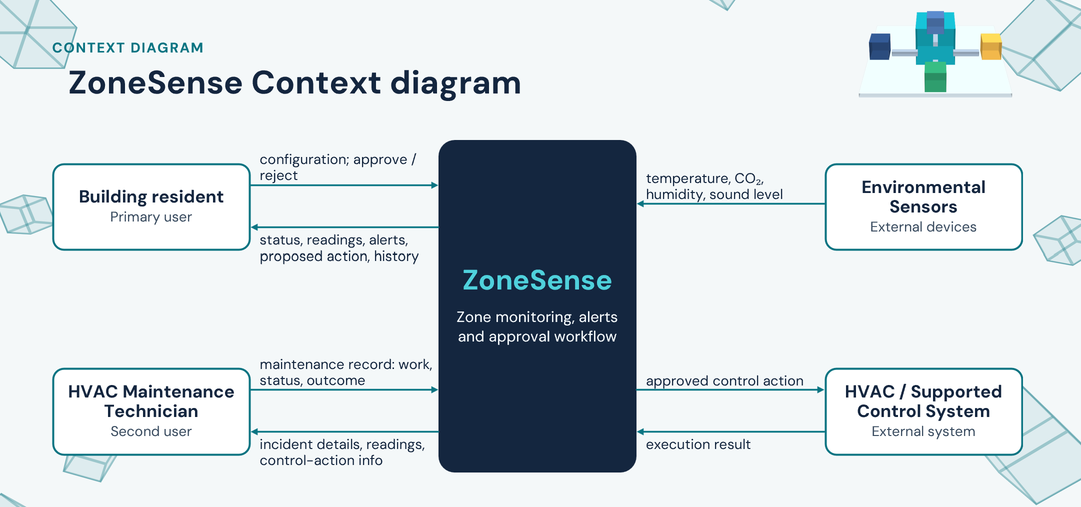
\includegraphics[width=\linewidth]{context_diagram.png}
  \caption{ZoneSense context diagram}
  \label{fig:context}
\end{figure}

% ---------------------------------------------------------------------
\clearpage
\section{Architectural Design and Design Patterns}

\subsection{System Context}
ZoneSense sits between three kinds of external parties: \textbf{people} (Building Resident, HVAC Maintenance Technician), \textbf{environmental sensors} that send readings, and the \textbf{HVAC / supported control system} that executes approved actions. The sensors and the HVAC system are simulated in the prototype. Databases and internal services are part of the system and therefore appear in the container diagram, not as actors.

\begin{figure}[H]
  \centering
  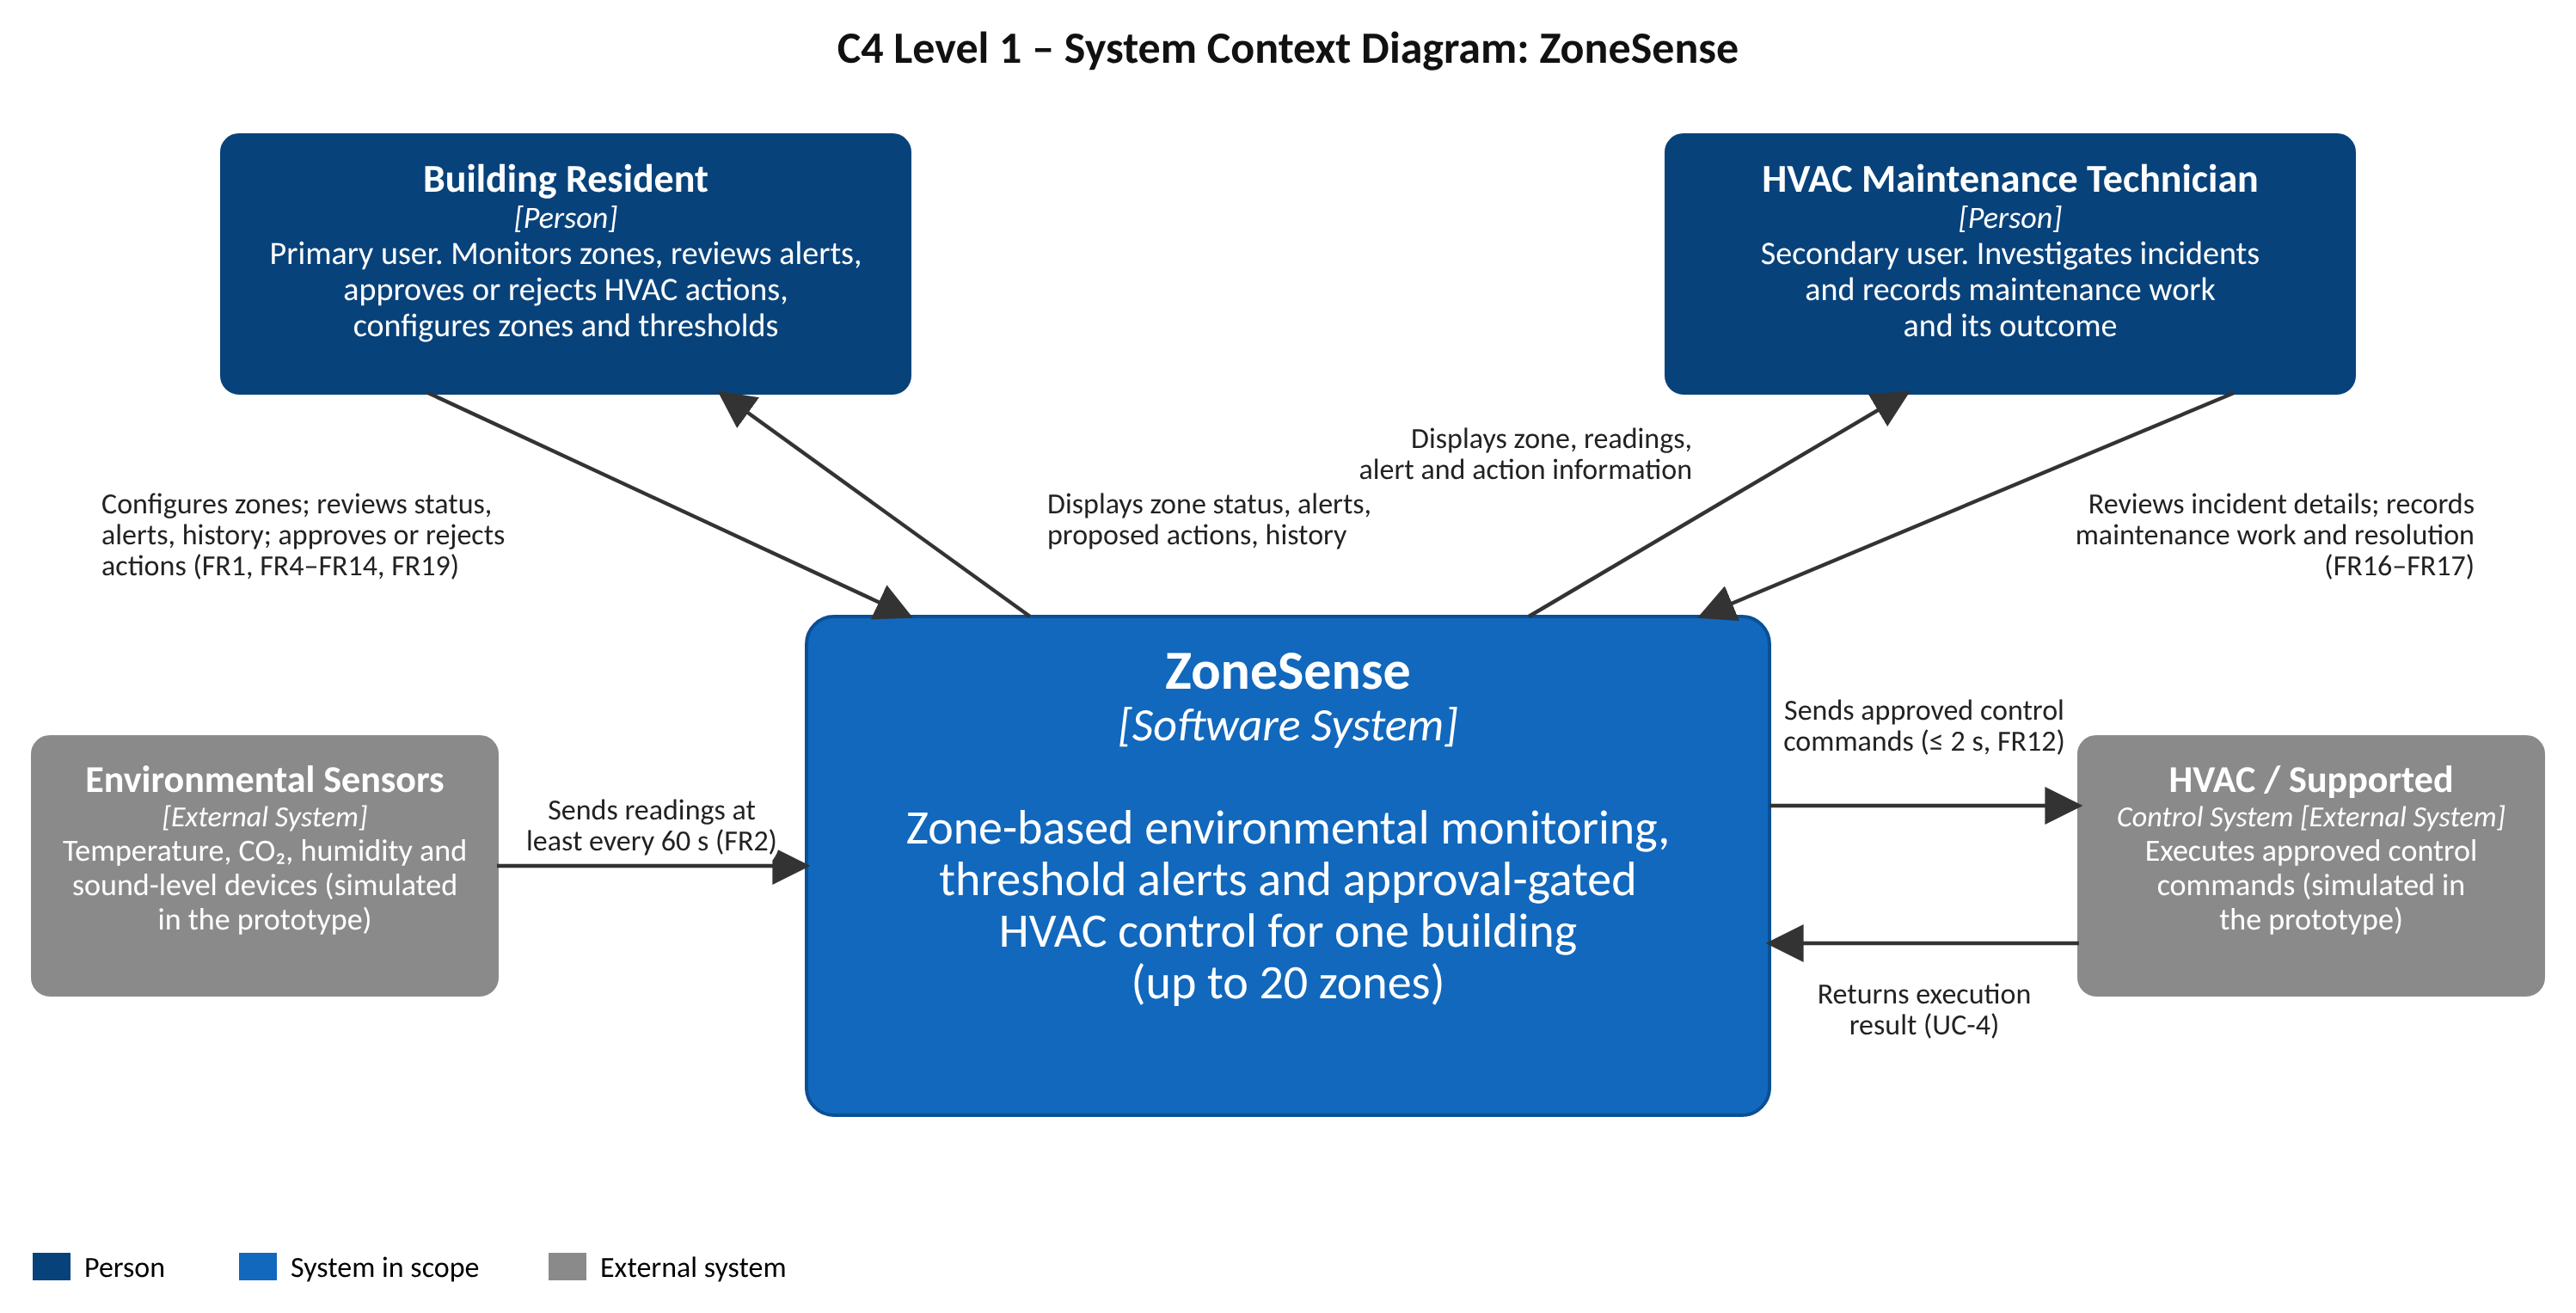
\includegraphics[width=\linewidth]{c4_context.png}
  \caption{C4 Level 1: System Context diagram}
  \label{fig:c4-context}
\end{figure}

\subsection{Architectural Proposal}
\textbf{Proposed style: layered modular monolith with internal event-driven alert handling.} ZoneSense is deployed as one application with four layers (presentation, application services, domain rules, data/integration). Alerts are published internally to subscribers (dashboard, control proposal, audit), so new reactions can be added without modifying the alert generator.

{\small\stripe
\begin{xltabular}{\linewidth}{|L{3.1cm}|Y|L{5.3cm}|}
\caption{Layers and their responsibilities}\label{tab:layers}\\
\hline\headrow
\hd{Layer} & \hd{Responsibility} & \hd{Components}\\\hline
\endfirsthead
\hline\headrow
\hd{Layer} & \hd{Responsibility} & \hd{Components}\\\hline
\endhead
Presentation & Web pages and REST endpoints for the Building Resident and the HVAC Maintenance Technician. Every request passes the authentication and role check first. & Web Application, REST API Controller, Authentication and Access Control\\\hline
Application services & Coordinate the use cases: receive readings, evaluate zones, raise and route alerts, propose, approve and record control actions, keep maintenance records. & Sensor Reading Service, Monitoring Service, Alert Manager, Control Proposal Service, Approval Service, Maintenance and History Service, Audit Logger\\\hline
Domain rules & Business rules that do not depend on the interface or on storage: thresholds, zone status, alert severity and the repeat-alert interval. & \code{ThresholdRule}, \code{RangeRule}, \code{UpperLimitRule}, \code{ZoneStatusEvaluator}\\\hline
Data and integration & Store data and talk to the outside world. & Repository Layer, relational database, HVAC Adapter\\\hline
\end{xltabular}}

{\small\stripe
\begin{xltabular}{\linewidth}{|L{3.6cm}|L{3.3cm}|Y|L{1.9cm}|}
\caption{Justification against alternatives}\label{tab:alternatives}\\
\hline\headrow
\hd{Option} & \hd{Advantages} & \hd{Disadvantages for ZoneSense} & \hd{Decision}\\\hline
\endfirsthead
\hline\headrow
\hd{Option} & \hd{Advantages} & \hd{Disadvantages for ZoneSense} & \hd{Decision}\\\hline
\endhead
Simple single-layer monolith & Fastest to build & Rules, UI and data become tangled; hard to replace simulated HVAC & Rejected\\\hline
Microservices & Independent scaling & Operational overhead is unjustified for 1 building, 80 streams and a student team & Rejected\\\hline
Broker-based event-driven & Decoupling at scale & Extra infrastructure; only $\sim$80 readings/min & Rejected for now\\\hline
\textbf{Layered modular monolith + internal events} & Simple deployment, clear modules, testable, extensible & Scales vertically only & \textbf{Selected}\\\hline
\end{xltabular}}

{\small\stripe
\begin{xltabular}{\linewidth}{|L{4.6cm}|Y|}
\caption{Quality attributes addressed}\label{tab:quality}\\
\hline\headrow
\hd{Requirement} & \hd{Architectural decision}\\\hline
\endfirsthead
\hline\headrow
\hd{Requirement} & \hd{Architectural decision}\\\hline
\endhead
NFR1, NFR2 (8 s / 45 s) & Readings evaluated on arrival; alerts published to subscribers in-process\\\hline
NFR3, NFR8 (availability, reliability) & Per-sensor monitoring; each observer isolated by exception handling\\\hline
NFR4, NFR5 (security) & Authentication and role check in one gateway layer before any service\\\hline
NFR6, FR18 (audit, 12 months) & Audit logger subscribes to every alert and decision; relational store\\\hline
FR22 (repeat-alert limit) & Alert Manager keeps the last alert per zone and measurement and suppresses unchanged repeats inside the configured interval\\\hline
NFR13 (encrypted transport) & HTTPS between browser and server; TLS for sensor ingestion and database connections; passwords stored hashed\\\hline
NFR11 (maintainability) & Thresholds stored as configuration, not code (Strategy)\\\hline
NFR12 (scalability) & Capacity: 80 readings/min = 115,200/day $\approx$ 42.0 million rows/year, well within a single relational database\\\hline
\end{xltabular}}

\subsubsection*{Trade-offs of the chosen style}
\textbf{Scalability.} The design grows by running on a bigger single server, not by adding services. This is enough because the specified maximum is 20 zones with 4 measurements each, 80 streams, about 80 readings per minute or 42.0 million rows per year, which one relational database can hold (NFR12). \textbf{Complexity.} One deployable application with in-process events has no network calls between modules, so a small team has only the application and its database to build, test and run within one semester. \textbf{Cost.} No message broker, container orchestration or extra servers are needed. \textbf{What we give up.} The application is a single point of failure, a heavy load in one module can slow the others, and parts cannot be scaled independently. If ZoneSense later covered many buildings, alert handling could move to a message broker. Because the modules already communicate through defined interfaces (events, repositories and the HVAC adapter), that step would not require redesigning the domain rules.

\subsection{C4 Level 2 -- Container Diagram}
\begin{figure}[H]
  \centering
  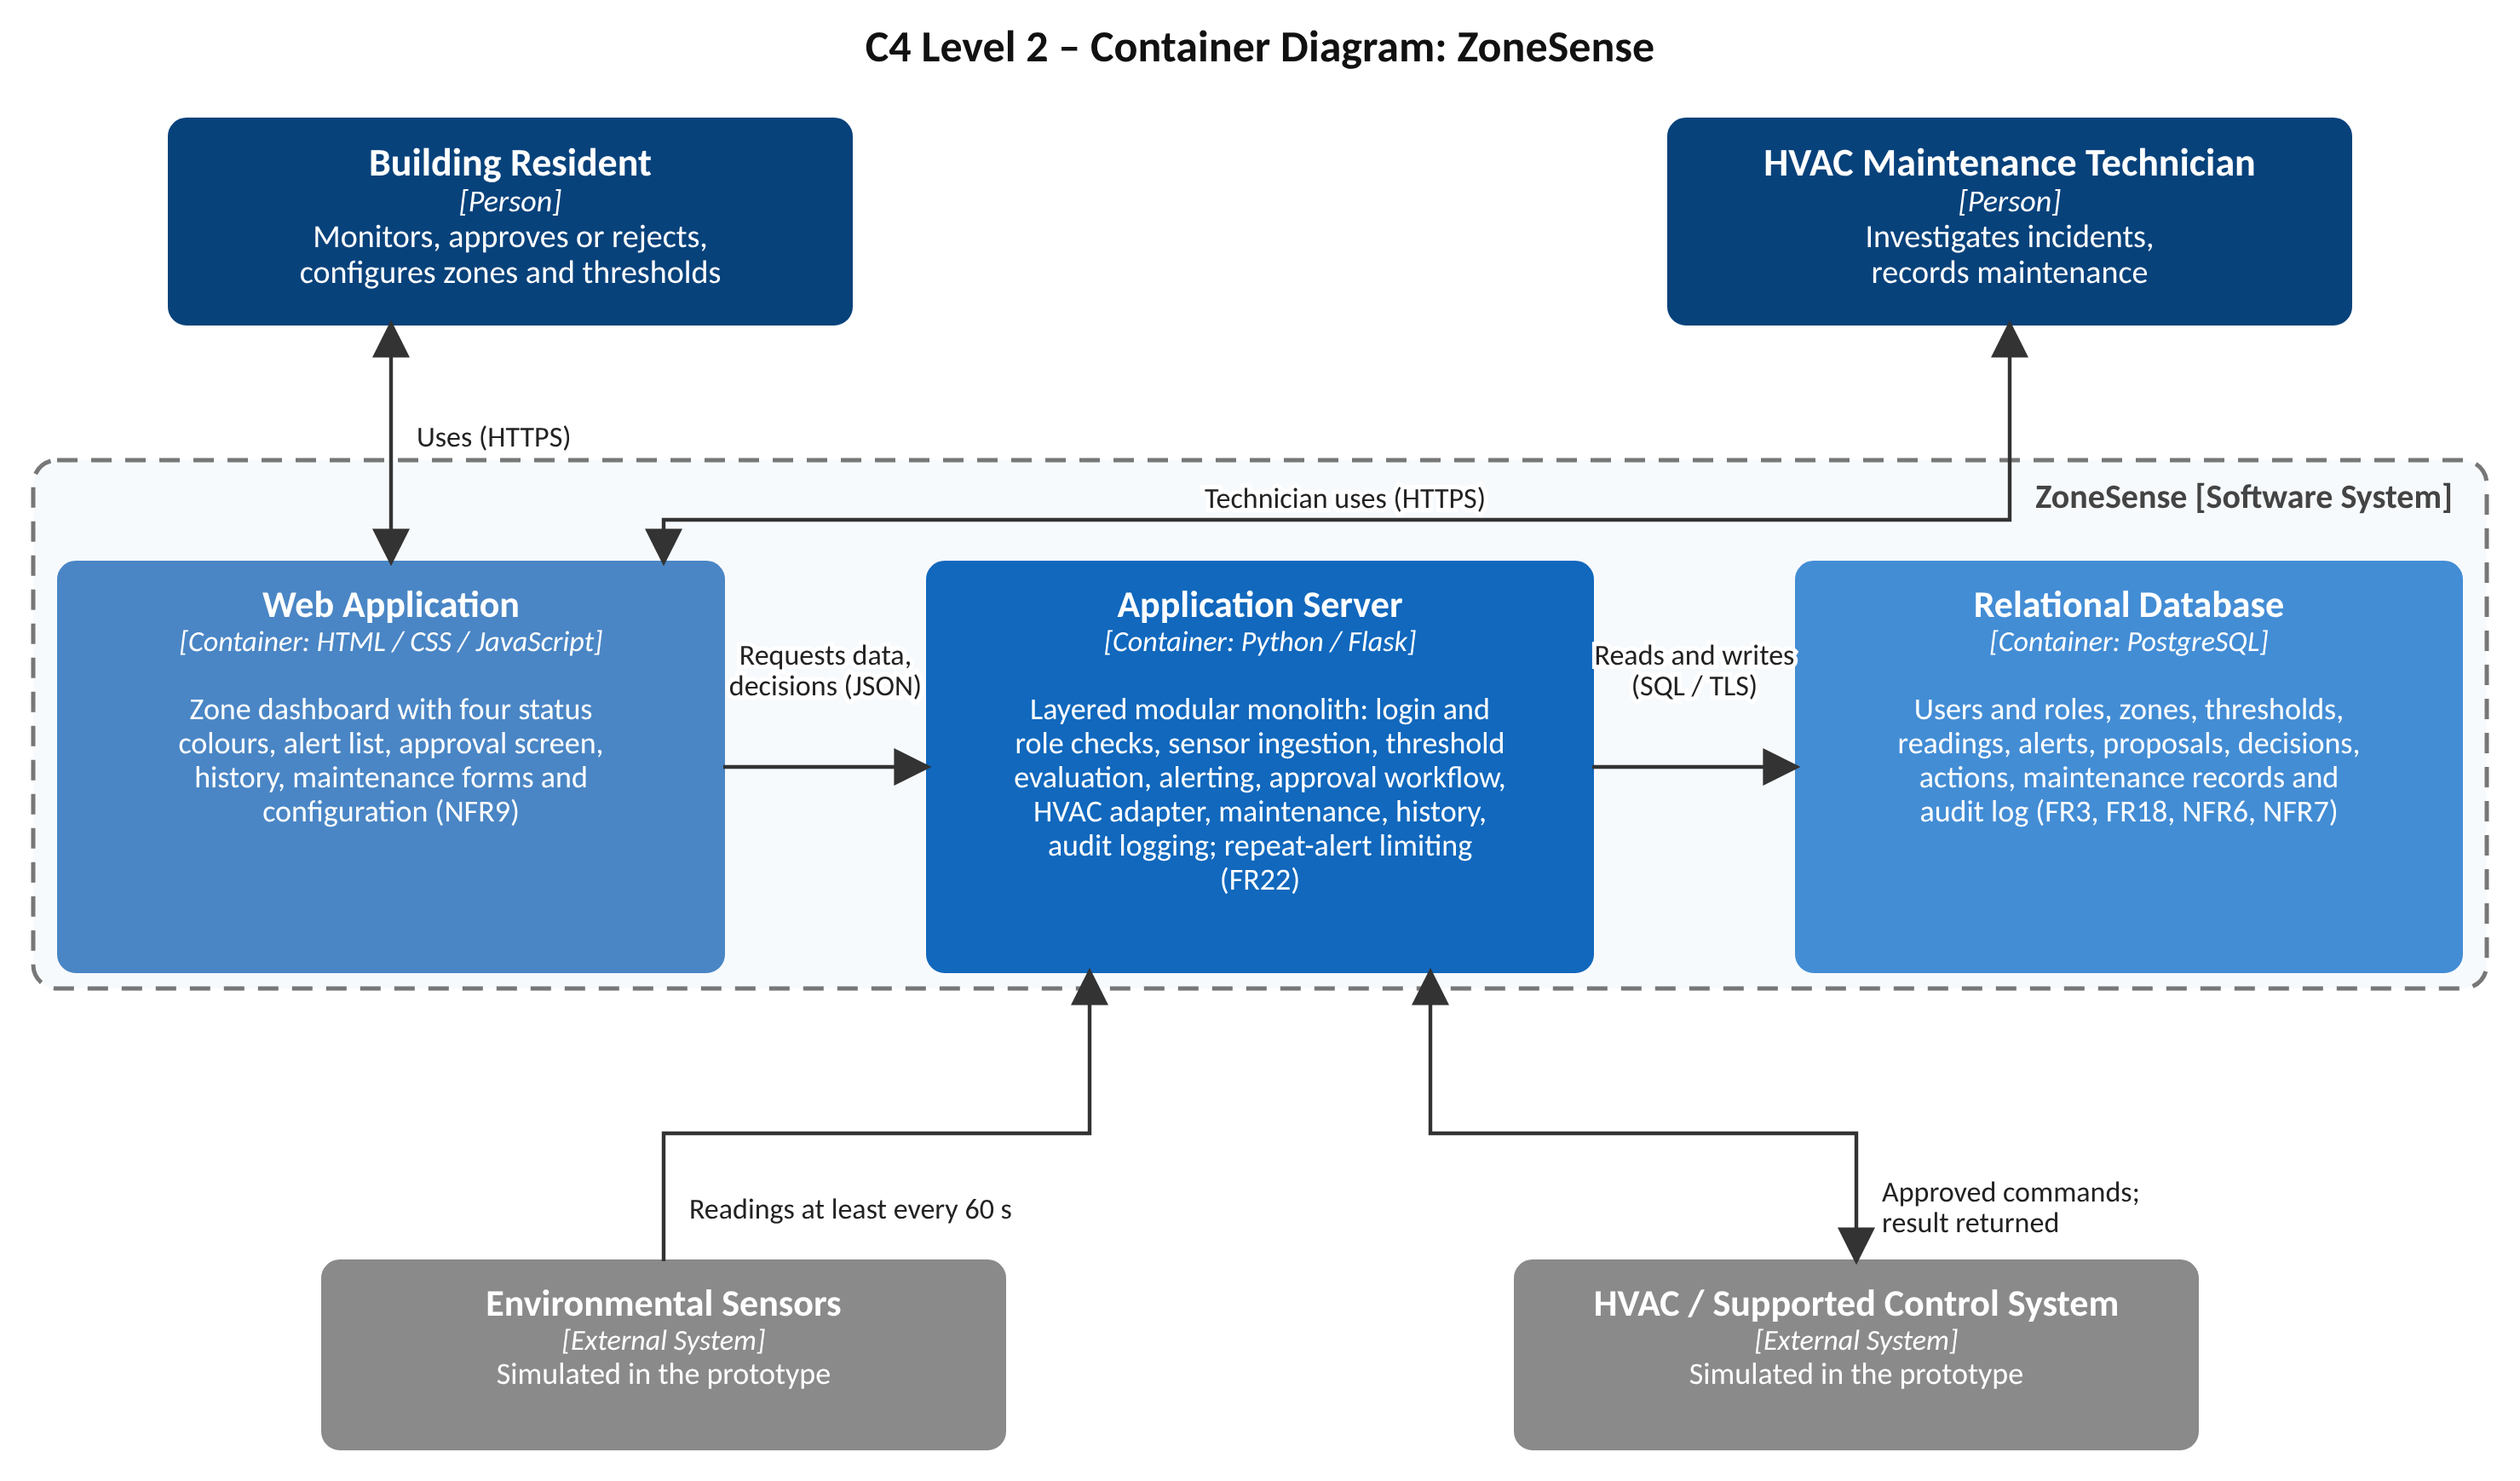
\includegraphics[width=\linewidth]{c4_container.png}
  \caption{C4 Level 2: Container diagram}
  \label{fig:c4-container}
\end{figure}

The Environmental Sensors external system includes the sensor gateway that forwards readings to ZoneSense; both are simulated in the prototype. The connection from the gateway to the Application Server, like the browser and database connections, uses TLS 1.2 or higher (NFR13).

\subsection{C4 Level 3 -- Component Diagram}
\begin{figure}[H]
  \centering
  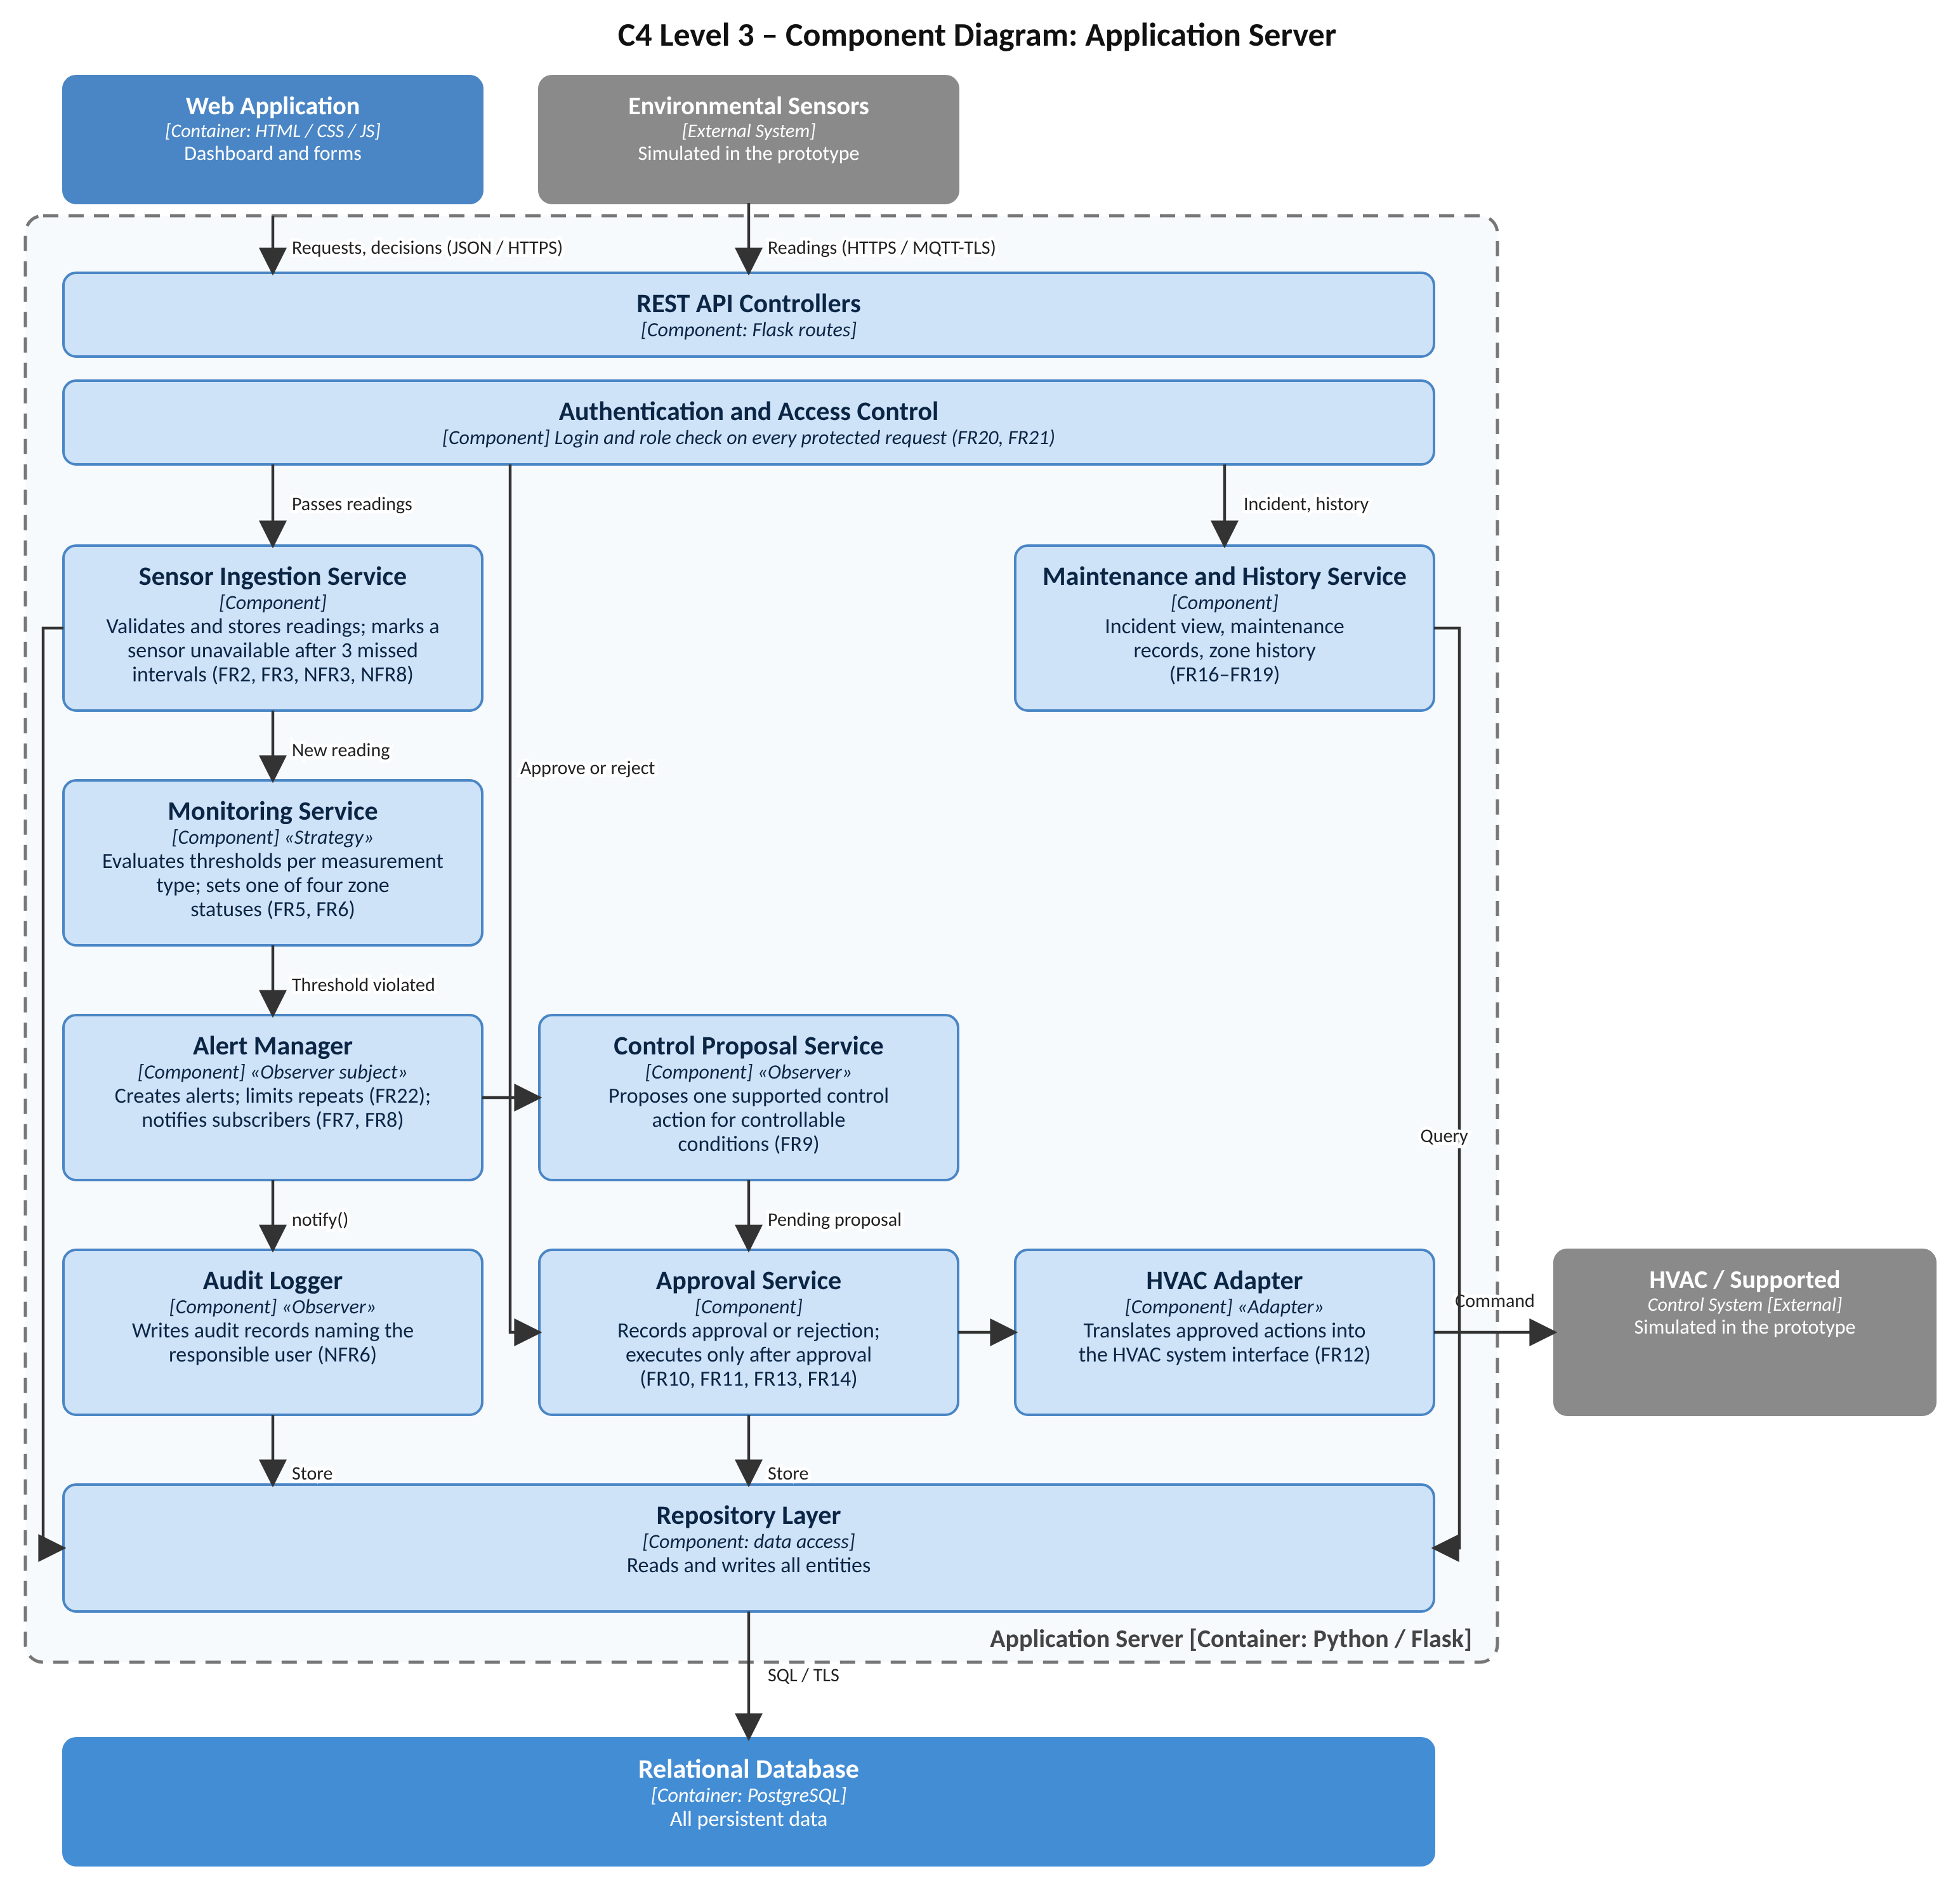
\includegraphics[width=\linewidth,height=0.72\textheight,keepaspectratio]{c4_component.png}
  \caption{C4 Level 3: Components of the ZoneSense application}
  \label{fig:c4-component}
\end{figure}

\subsection{Design Patterns}
Three Gang-of-Four patterns are applied where the requirements create real variation. Code is shown in Python; the prototype output follows each section.

% ---------- Pattern 1 ----------
\subsubsection*{Pattern 1 -- Strategy (threshold evaluation, FR5, FR6, NFR11)}
\textbf{Problem:} temperature and humidity are out of range on both sides, while \COtwo{} and sound are only limited from above; thresholds must change without editing code. \textbf{Solution:} each measurement gets a \code{ThresholdRule} strategy; \code{ZoneStatusEvaluator} selects it. \textbf{Principles:} Open/Closed, Single Responsibility.

\begin{figure}[H]
  \centering
  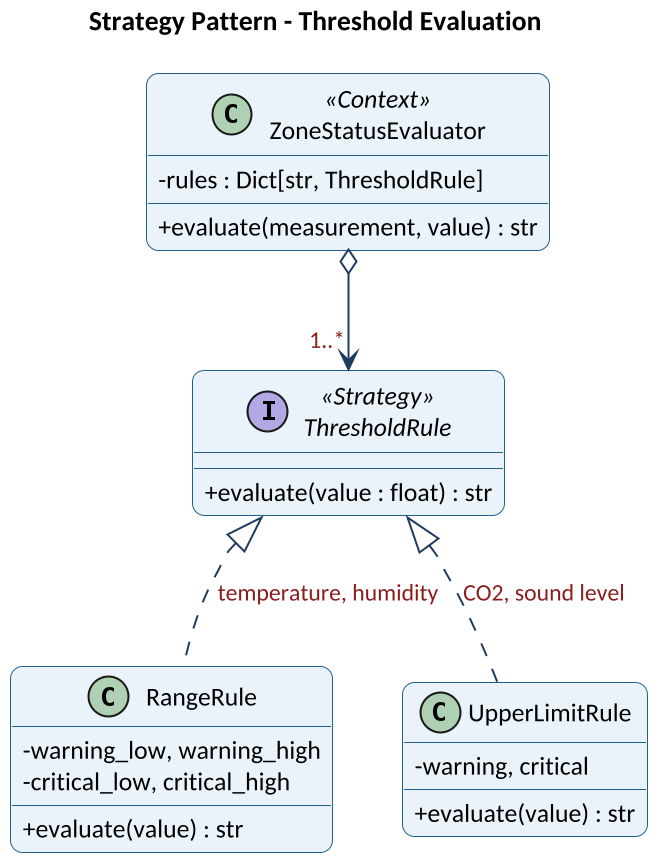
\includegraphics[width=0.48\linewidth]{strategy_uml.png}
  \caption{Strategy pattern UML}
  \label{fig:strategy}
\end{figure}

\begin{lstlisting}
# ---------- Strategy: threshold evaluation (FR5, FR6, NFR11) ----------
class ThresholdRule(ABC):
    @abstractmethod
    def evaluate(self, value: float) -> str: ...

class RangeRule(ThresholdRule):          # temperature, humidity
    def __init__(self, warning_low, warning_high, critical_low, critical_high):
        self.wl, self.wh, self.cl, self.ch = warning_low, warning_high, critical_low, critical_high
    def evaluate(self, value):
        if value < self.cl or value > self.ch: return "critical"
        if value < self.wl or value > self.wh: return "warning"
        return "normal"

class UpperLimitRule(ThresholdRule):     # CO2, sound level
    def __init__(self, warning, critical): self.w, self.c = warning, critical
    def evaluate(self, value):
        return "critical" if value >= self.c else "warning" if value >= self.w else "normal"

class ZoneStatusEvaluator:
    def __init__(self, rules): self.rules = rules
    def evaluate(self, measurement, value): return self.rules[measurement].evaluate(value)
\end{lstlisting}

% ---------- Pattern 2 ----------
\subsubsection*{Pattern 2 -- Observer (alert notification, FR7, FR8, FR22, NFR6)}
\textbf{Problem:} one alert must reach the dashboard, the control-proposal logic and the audit log, and new subscribers should not change the alert generator. \textbf{Solution:} \code{AlertManager} (subject) notifies subscribed \code{AlertObserver}s; a failing observer cannot block the others. \textbf{Principles:} Open/Closed, loose coupling.

\begin{figure}[H]
  \centering
  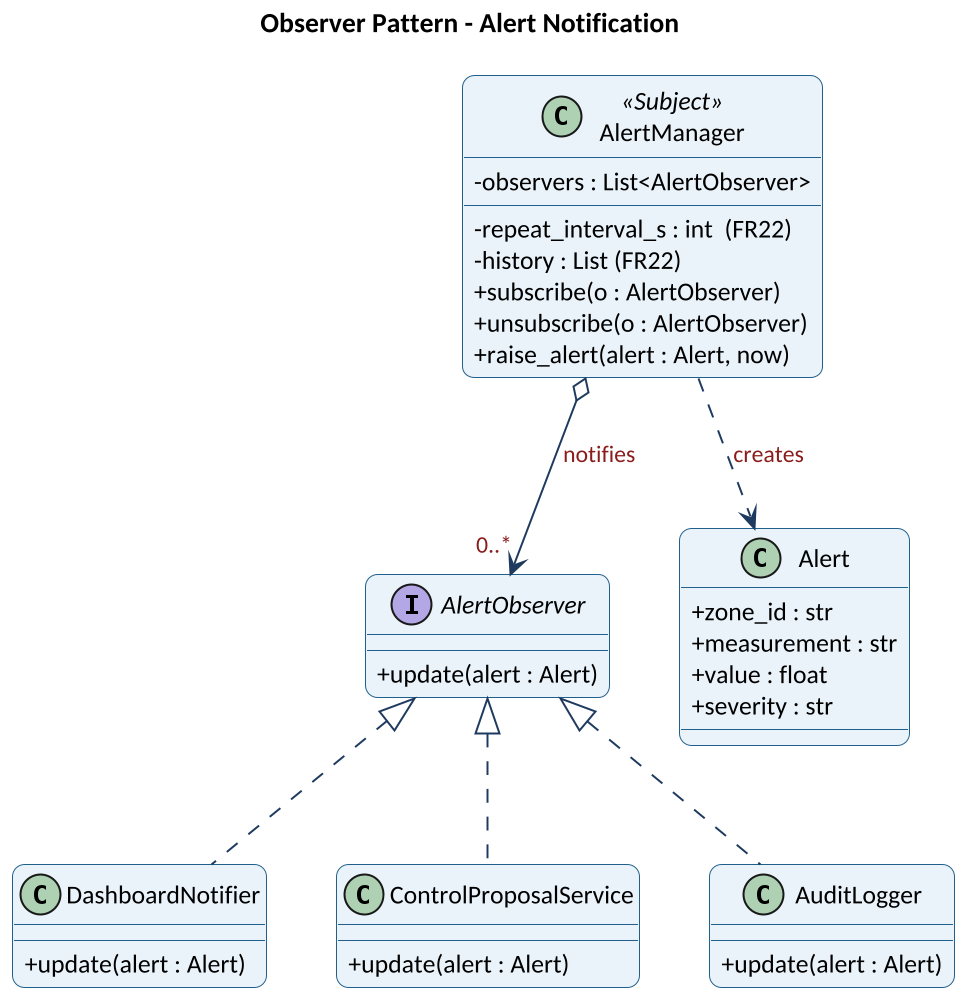
\includegraphics[width=0.62\linewidth]{observer_uml.png}
  \caption{Observer pattern UML}
  \label{fig:observer}
\end{figure}

\begin{lstlisting}
# ---------- Observer: alert notification (FR7, FR8, FR22, NFR6) ----------
@dataclass
class Alert:
    zone_id: str; measurement: str; value: float; severity: str

class AlertObserver(ABC):
    @abstractmethod
    def update(self, alert: Alert) -> None: ...

class AlertManager:
    def __init__(self, repeat_interval_s=600):          # default 10 min
        assert 60 <= repeat_interval_s <= 3600           # FR22: 1-60 minutes
        self._observers, self._last, self.interval = [], {}, repeat_interval_s
        self.history = []                                # FR22: suppressed repeats are stored
    def subscribe(self, o): self._observers.append(o)
    def unsubscribe(self, o): self._observers.remove(o)
    def clear(self, zone_id, measurement):               # FR22: a normal reading ends the episode
        self._last.pop((zone_id, measurement), None)
    def raise_alert(self, alert, now=0):
        key = (alert.zone_id, alert.measurement)
        last = self._last.get(key)
        if last and last[1] == alert.severity and now - last[0] < self.interval:
            self.history.append((now, alert, "suppressed repeat"))               # FR22: stored in history
            print(f"[AlertManager] repeat suppressed and stored: {key} {alert.severity}")
            return
        self._last[key] = (now, alert.severity)
        self.history.append((now, alert, "alert shown"))
        for o in self._observers:
            try: o.update(alert)
            except Exception as e: print(f"[AlertManager] {type(o).__name__} failed: {e}")

class DashboardNotifier(AlertObserver):
    def update(self, a): print(f"[Dashboard]  {a.severity.upper()} alert: {a.zone_id} {a.measurement}={a.value}")
class ControlProposalService(AlertObserver):
    def update(self, a):                                  # simplified: FR9 covers any supported abnormal condition
        if a.severity == "critical": print(f"[Proposal]   HVAC action proposed for {a.zone_id} (awaiting approval)")
class AuditLogger(AlertObserver):
    def update(self, a): print(f"[Audit]      logged {a.severity} {a.measurement} event in {a.zone_id}")
\end{lstlisting}

% ---------- Pattern 3 ----------
\subsubsection*{Pattern 3 -- Adapter (HVAC integration, FR9--FR13)}
\textbf{Problem:} the prototype uses simulated HVAC, but a real vendor interface has a different API that must not leak into the approval logic. \textbf{Solution:} \code{ApprovalService} depends on the \code{HVACController} interface; \code{VendorHVACAdapter} wraps the vendor API and \code{SimulatedHVACAdapter} serves the prototype. The service executes only approved proposals (FR10, FR13). \textbf{Principles:} Dependency Inversion, Open/Closed.

\begin{figure}[H]
  \centering
  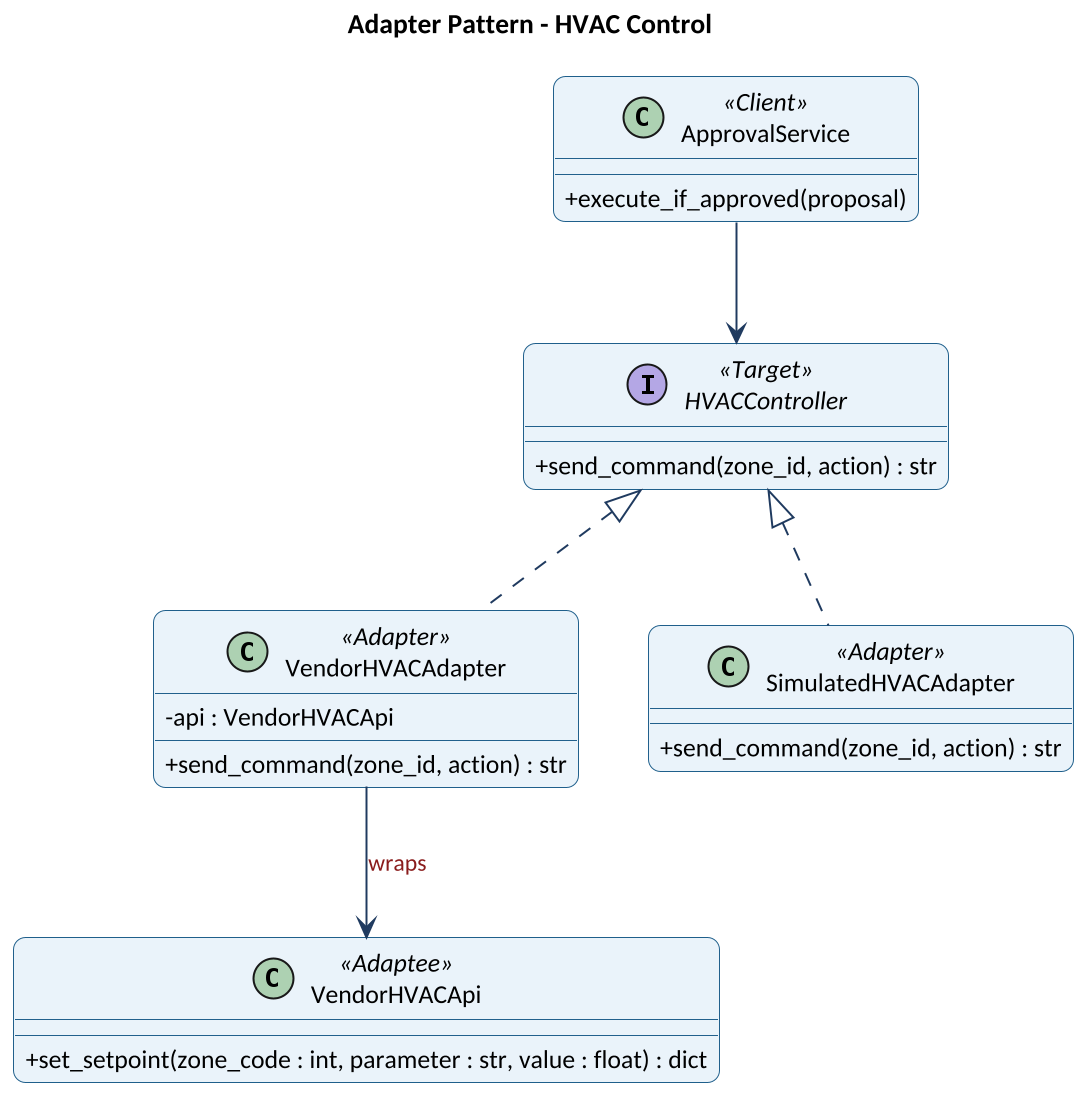
\includegraphics[width=0.62\linewidth]{adapter_uml.png}
  \caption{Adapter pattern UML}
  \label{fig:adapter}
\end{figure}

\begin{lstlisting}
# ---------- Adapter: HVAC control (FR10, FR12, FR13) ----------
class HVACController(ABC):
    @abstractmethod
    def send_command(self, zone_id: str, action: str) -> str: ...

class VendorHVACApi:                      # third-party interface we cannot change
    def set_setpoint(self, zone_code: int, parameter: str, value: float) -> dict:
        return {"zone": zone_code, "param": parameter, "value": value, "ack": True}

class VendorHVACAdapter(HVACController):
    ACTIONS = {"increase_ventilation": ("fan_speed", 80.0), "reduce_cooling": ("temp_setpoint", 24.0)}
    def __init__(self, api): self.api = api
    def send_command(self, zone_id, action):
        param, value = self.ACTIONS[action]
        r = self.api.set_setpoint(int(zone_id.lstrip("Z")), param, value)
        return f"vendor ack={r['ack']} ({param}={value})"

class SimulatedHVACAdapter(HVACController): # prototype
    def send_command(self, zone_id, action): return f"simulated '{action}' applied to {zone_id}"

class ApprovalService:
    def __init__(self, controller): self.controller = controller
    def execute_if_approved(self, zone_id, action, approved):
        return self.controller.send_command(zone_id, action) if approved else "rejected - no command sent"
\end{lstlisting}

% ---------- Demonstration ----------
\subsubsection*{Demonstration and output}
\begin{lstlisting}
ev = ZoneStatusEvaluator({"co2": UpperLimitRule(1000, 1500), "temperature": RangeRule(20, 26, 18, 30)})
mgr = AlertManager()
for o in (DashboardNotifier(), ControlProposalService(), AuditLogger()): mgr.subscribe(o)
for z, m, v in [("Z03", "co2", 1620), ("Z07", "temperature", 27.5), ("Z01", "co2", 640)]:
    s = ev.evaluate(m, v); print(f"{z} {m}={v} -> {s}")
    if s != "normal": mgr.raise_alert(Alert(z, m, v, s))
    else: mgr.clear(z, m)
mgr.raise_alert(Alert("Z03", "co2", 1650, "critical"), now=120)   # same condition, 2 min later
mgr.raise_alert(Alert("Z03", "co2", 1650, "critical"), now=900)   # after the 10-min interval
print("History entries:", len(mgr.history), "(", sum(1 for h in mgr.history if h[2]=="suppressed repeat"), "suppressed repeat )")
print()
for ctrl in (SimulatedHVACAdapter(), VendorHVACAdapter(VendorHVACApi())):
    svc = ApprovalService(ctrl)
    print(type(ctrl).__name__, "->", svc.execute_if_approved("Z03", "increase_ventilation", True))
print("Rejected ->", ApprovalService(SimulatedHVACAdapter()).execute_if_approved("Z03", "increase_ventilation", False))

# Output
Z03 co2=1620 -> critical
[Dashboard]  CRITICAL alert: Z03 co2=1620
[Proposal]   HVAC action proposed for Z03 (awaiting approval)
[Audit]      logged critical co2 event in Z03
Z07 temperature=27.5 -> warning
[Dashboard]  WARNING alert: Z07 temperature=27.5
[Audit]      logged warning temperature event in Z07
Z01 co2=640 -> normal
[AlertManager] repeat suppressed and stored: ('Z03', 'co2') critical
[Dashboard]  CRITICAL alert: Z03 co2=1650
[Proposal]   HVAC action proposed for Z03 (awaiting approval)
[Audit]      logged critical co2 event in Z03
History entries: 4 ( 1 suppressed repeat )

SimulatedHVACAdapter -> simulated 'increase_ventilation' applied to Z03
VendorHVACAdapter -> vendor ack=True (fan_speed=80.0)
Rejected -> rejected - no command sent
\end{lstlisting}

\begin{zcallout}
\textbf{Illustrative code versus the real design.} The in-memory \code{history} list and the Boolean \code{approved} argument only demonstrate the patterns, and the demo proposes an HVAC action only for critical alerts, whereas FR9 covers any supported abnormal temperature, \COtwo{} or humidity condition. In the real design, alerts, suppressed repeats and approval decisions are stored in the relational database for at least 12 months (FR18), and an approval is an authenticated, role-checked and audited action by an authorized Building Resident (FR14, FR20, FR21, NFR6).
\end{zcallout}

\subsection{Summary}
The layered modular monolith is designed to meet the specified performance, security and audit requirements with the least complexity for a single building of up to 20 zones. Strategy keeps thresholds configurable, Observer decouples alert handling, and Adapter isolates the HVAC vendor. The design can later be split into services if the project grows beyond one building.

\end{document}
